% (g) Popis metodiky testování a jeho výsledky.
% (h) Srovnání s podobnými implementacemi (pokud existují).

\chapter{Testování}
Testování (\textit{testing}) provázelo vzniklé aplikace po celou dobu vývoje -- od evaluace požadavků na počátku, až po akceptační testy na konci. Testování probíhala, byť v jinou dobu, obdobně u serverové i mobilní aplikace, pro větší přehlednost jejich popis tedy sloučím.

\section{Funkční testování}
Funkční testování (\textit{functional testing}) reprezentuje skupinu různorodých testů, které ověřují, zda byly splněny všechny funkční požadavky na systém. Jeho výsledky jsou tedy zpravidla velmi kategorické. Nevyužil jsem proto formálních metodik -- jejich závěry by měly být shodné s těmi mými založenými na prosté důkladné kontrole projektu.

\subsection{Testování programátorem}
Testování programátorem zahrnuje širokou skupinu testů prováděných přímo programátorem v průběhu vývoje. Patří mezi ně jednotkové testování (\textit{unit testing}), revize kódu (\textit{code review}), testování mezních hodnot (\textit{boundary testing})\dots

Každou přidávanou jednotku jsem testoval mezními hodnotami. V průběhu vývoje jsem opakovaně revidoval v předchozích iteracích napsaný kód a v~případě potřeby ho komentoval a refaktoroval pro větší kvalitu (lepší čitelnost, deduplikakace, zjednodušení\dots). Tato činnost sloužila k eliminaci lokálních chyb v kódu a přinášela pozitivní výsledky. Po změně vždy proběhlo nutné otestování, zda opravou nebyla zanesena další chyba.

% nefungující SPARQL v Chrome - špatný parametr accepts (místo {json: 'application/json'} pouze 'application/json')
% zbytečné zelenění
% mezní hodnoty

% \subsection{Testování funkcionalit}
% (\textit{feature testing}) moc se nepoužívá, neuvádím
% \todo{Splnění požadavků bylo testováno mnou i vedoucím práce.}

\subsection{Integrační testování}
Integrační testování (\textit{integration testing}) bylo prováděno u všech vyvíjených aplikací. Po přidání nové funkcionality byla vždy příslušná část aplikace důkladně otestována, aby bylo zamezeno situacím, kdy nově zanesené úpravy poškodí již existující funkcionality aplikace -- takto vzniklé a neošetřené chyby totiž bývají velmi záludné -- vývojář otestoval všechny části, nenalezl v nich žádný problém, takže je považuje za korektní, možnost chyb daných integrací ho nenapadne a při pozdějším výskytu problému pak hledá řešení na špatných místech, protože skutečné místo považuje za již důkladně otestované.

\subsection{Akceptační testování}
Akceptační testování (\textit{acceptance testing}) ověřuje, zda byly do požadované míry naplněny všechny požadavky a po jeho úspěšném dokončení je systém zpravidla předán.

Akceptační testování bylo prováděno bez formální metodiky vedoucím práce, inženýrem Havrylukem, a mnou, jako osobou mající největší zájem na úspěšném naplnění všech požadavků. Systém byl akceptován.


\section{Nefunkční testování}
Nefunkční testování (\textit{non-functional testing}) zahrnuje skupinu testů ověřujících naplnění nefunkčních požadavků na systém. Zde se z principu očekávají výsledky více vágní, než v případě funkčního testování, proto jsem také věnoval podstatně více času na provedení formalizovanějších testů. Jeho výsledky by měly korelovat s kvalitou vytvořeného produktu.

\subsection{Testování kompatibility}
\label{sec:test:compat}
Testování kompatibility (\textit{compatibility testing}) je proces ověřující správný chod systému v různých prostředích -- zařízeních, operačních systémech, běhových prostředích\dots Serverová aplikace je nasazena na konkrétním serveru a s častým přemisťováním se nepočítá, věnovat se proto budu v této sekci pouze mobilní aplikaci, která je na tom přesně opačně -- bude nasazena na zařízeních uživatelů, která jsou vzájemně dosti odlišná.

\subsubsection{Charakteristika testu}
Testování bylo v omezeném počtu prohlížečů prováděno po celou dobu vývoje, ve zbylých až v době finalizace. Testovalo se v prohlížečích:
\begin{itemize}
 \item Mozilla Firefox (\url{http://www.mozilla.org/firefox/}).
 \item Chromium (\url{http://chromium.org/}).\footnote{Chromium je základem prohlížeče Google Chrome, dá se tedy předpokládat, že ten bude aplikaci podporovat na stejné úrovni.}
 \item Rekonq (\url{http://rekonq.kde.org/}).
 \item Konqueror (\url{http://www.konqueror.org/}).
 \item Internet Explorer (\url{http://ie.microsoft.com/}).
 \item Prohlížeč platformy Android (\url{http://android.com/}).\footnote{Verze 2 a 4.}
 \item Opera Mobile (\url{http://www.opera.com/mobile/}).
 \item Opera Mini (\url{http://www.opera.com/mini/}).
 \item Internet Explorer Mobile (\url{http://www.microsoft.com/windowsphone/en-us/features/default.aspx#internet-explorer}).
\end{itemize}
Mimo výše uvedených navíc nabídl pan inženýr Havryluk, vedoucí práce, otestování v následujících prohlížečích:
\begin{itemize}
 \item Google Chrome for Android (\url{https://www.google.com/intl/en/chrome/android/}).
 \item Prohlížeč platformy Android (\url{http://android.com/}).\footnote{Verze 3.}
%  \item Dolphin Browser (\url{http://dolphin-browser.com/}).
%  \item Nokia Browser for Symbian  (\url{http://browser.nokia.com/}).
%  \item Prohlížeč platformy BlackBerry (\url{http://us.blackberry.com/smartphones/features/internet.jsp}).
%  \item Safari (\url{http://www.apple.com/safari/}).
\end{itemize}


\subsubsection{Průběh a shrnutí testu}
V následující části jsou popsány nalezené problémy jednotlivých prohlížečů, pokud není uvedené jinak, aktuálních verzí:
\subsubsection*{Mozilla Firefox}
Mozilla Firefox po pozměnění vynucuje překreslení \glsname{SVG}, které je navíc poměrně pomalé, snažil jsem se proto algoritmy upravit tak, aby \glsname{SVG} zbytečně nepozměňovaly. Jinak vše funguje, jak má.

\subsubsection*{Chromium}
Nelze nastavit transformaci \glsname{SVG} elementu, problém ale lze obejít méně elegantním způsobem. Vše funguje, jak má.

\subsubsection*{Rekonq}
Prohlížeč nepodporuje geolokační \glsname{API}, takže nelze určit polohu uživalete. Prohlížeč také výchozím fontem zobrazuje velmi úzké bílé znaky, takže nemusí být tolik přehledné formátování například ve \glsname{SPARQL} konzoli. Jinak vše funguje, jak má.

\subsubsection*{Konqueror}
Prohlížeč ve výchozím \textit{renderovacím} jádru, KHTML, nepodporuje přímé vkládání \glsname{SVG} do \glsname{HTML}, nefunguje v něm tedy navigace -- uživatel je na toto omezení upozorněn. Jinak vše funguje, jak má.

\subsubsection*{Internet Explorer}
Do verze 9 neměl Internet Explorer bez přidaných rozšíření dostatečnou podporu \glsname{SVG} a nepodporoval tak navigaci; od verze 9, včetně, je vše v pořádku. V tomto prohlížeči jsem také narazil na chybu oproti specifikaci ECMAScriptu:\footnote{Jazyk JavaScript je z právních důvodů standardizován pod názvem ECMAScript, v~ptáci se držím více zažitého názvu.} není zde povoleno pojmenovat vlastnost objektu rezervovaným slovem \texttt{default}, což by mělo být zakázané pouze na místech označených jako \textit{Identifiers}, nikoliv tedy jako \textit{Identifier Names} \cite{JsIdentifiers}, přejmenování proměnné zde problém vyřešilo. Jinak vše funguje, jak má.

\subsubsection*{Opera}
V Opeře se při vyhledávání v rámci navigace nezobrazovaly objekty uvnitř budov, nejprve jsem z toho velmi chybně vinil špatnou implementaci průhlednosti,\footnote{Nejprve jsem se s tímto problémem setkal u Opera Mobile, kde by to bylo pochopitelné.} po dlouhém zkoumání jsem ale zjistil, že Opera nedokáže v některých případech vlivem odlišného \glsname{DOM} \glsname{SVG} pracovat přímo se třídami \glsname{SVG} elementů, ale musí se k jejich hodnotám v \glsname{DOM} přistupovat skrze delší cestu -- většina ostatních prohlížečů si s tímto problémem poradila. Problematické algoritmy byly přepracovány a problém odstraněn. Vše funguje, jak má.

\subsubsection*{Prohlížeč platformy Android}
Do verze 2, včetně, nepodporuje prohlížeč \glsname{SVG} -- tudíž nefunguje navigace, to se ale ve verzích 3 a 4 změnilo a podpora celé aplikace je tak bezproblémová. Vše funguje, jak má.

\subsubsection*{Opera Mobile}
V Opeře Mobile se vyskytoval stejný problém, jaký byl odhalen u \textit{desktopové} verze -- nezobrazovaly se objekty uvnitř budov. Odstraněním problému v \textit{desktopové} verzi byl odstraněn i zde. Vše funguje, jak má.

\subsubsection*{Opera Mini}
Prohlížeč Opera Mini nepodporuje přímé vkládání \glsname{SVG} do \glsname{HTML}, nefunguje v něm tedy navigace -- uživatel je na toto omezení upozorněn. Také tento prohlížeč nedokáže zobrazit tabulátor v textových polích, například ve \glsname{SPARQL} konzoli -- byly tedy nahrazeny za mezery. Jinak vše funguje, jak má.

\subsubsection*{Internet Explorer Mobile}
Testována byla pouze verze 6, v té ještě nebyla přidána podpora \glsname{SVG}, která je již v aktuální verzi přítomná -- v testované verzi tedy nefunguje navigace. Také se zde projevovala, jako v \textit{desktopové} verzi, již opravená, chybná implementace omezení rezervovaných slov. Jinak vše funguje, jak má.

\subsubsection*{Google Chrome for Android}
Google Chrome for Android je teprve v betaverzi a některé věci tak ještě nejsou úplně odladěné. V aplikaci se projevila chyba, jinak velmi užitečné, funkce pro automatické přibližování v reakci na stisknutí odkazu -- uživateli by tak mělo být usnadněno jeho finální potvrzení, aniž by byl omylem aktivován jiný odkaz v blízkosti zamýšleného, v tomto případě je ale pouze zvětšováno a odkaz nelze vyvolat. Zdá se, že jinak vše funguje, jak má.


\subsection{Výkonnostní testování}
Výkonnostní testování (\textit{performance testing}) se zabývá, jak již název napovídá, testováním odezvy a stability systému za určitého zatížení. Lze ho dělit na zátěžové testování (\textit{load testing}), \textit{stress} testy\footnote{Český ekvivalent anglického \textit{stress} se v tomto případě pravděpodobně nevyužívá.}, testování výdrže (\textit{endurance testing}), testování konfigurací (\textit{configuration testing})\dots

Výkonnostní testování má smysl provádět jen na větších systémech dostupných většímu počtu potencionálních uživatelů -- což je v případě této práce pouze \glsname{SPARQL} endpoint \textit{serverové aplikace}.

Pro testování \glsname{SPARQL} endpointů jsou zpravidla využívány tyto \textit{benchmarky}:

\begin{itemize}
 \item \glsfirst{LUBM}\\ (\url{http://swat.cse.lehigh.edu/projects/lubm/})
 \item \glsfirst{SP2B}\\ (\url{http://dbis.informatik.uni-freiburg.de/?project=SP2B})
 \item \glsfirst{BSBM}\\ (\url{http://www4.wiwiss.fu-berlin.de/bizer/BerlinSPARQLBenchmark/})
\end{itemize}

První jmenovaný \textit{benchmark} pochází z Lehigh University, poslední verze je přibližně z roku 2005 a testování probíhá v doméně univerzity, tedy přesně v té, kterou potřebujeme. Pro potřeby tohoto \textit{benchmarku} vznikla ontologie zkoumaná v části \ref{sec:ontol:lubm} na straně \pageref{sec:ontol:lubm}.

Druhý jmenovaný pochází z Universität Freiburg, poslední verze je z roku 2009 a testování probíhá v doméně počítačové bibliografie, která je doméně našeho systému alespoň vzdáleně blízká.

Poslední jmenovaný pochází z Freie Universität Berlin, aktuální verze je z~roku 2011 a testování probíhá v doméně elektronického obchodního systému.

Po hrubém prozkoumání jmenovaných \textit{benchmarků} jsem se rozhodl vydat jinou cestou -- vytvořit si vlastní jednoduchý test zkoumající pouze chování \glsname{SPARQL} endpointu v zatížení o několik řádů větším, než maximálním předpokládaném. Výše uvedené \textit{benchmarky} mi tedy nakonec posloužily pouze jako zdroj inspirace, přesto je zde nechávám případným zájemcům pro pozdější podrobnější přezkoumání.

\subsubsection{Charakteristika testu}
K testování byl použit jednoduchý konzolový nástroj ApacheBench (\url{http://httpd.apache.org/docs/2.4/programs/ab.html}), jehož prostřednictvím byl \glsname{SPARQL} endpoint vystavován kontinuální paralelní zátěži. Tento nástroj stačil pouze po nějakou dobu -- v případě extrémních testů se projevilo jeho historické omezení -- umožňuje práci pouze s protokolem \glsname{HTTP} 1.0, zatímco Node.js, nad kterým je postavený \glsname{SPARQL} endpoint, naopak využívá perzistentní připojení \glsname{HTTP} 1.1, takže v ApacheBench dojde po nějaké době k~vypršení jednoho z několika vnitřních časových limitů a následnému ukončení.

\glsname{SPARQL} endpoint byl pro potřeby testování umístěn na virtuálním stroji řešení VirtualBox (\url{http://www.virtualbox.org/}) o jednom procesoru frekvence 2~GHz, 2~GB operační paměti a dostatečně rychlém síťovém připojení k hostitelskému počítači, ze kterého byly testy spouštěny.

Testy byly prováděny na bázi dat obsahující všechna data dostupná prostřednictvím implementovaných obsluhovačů zdrojů, nebylo prováděno \textit{cachování} a dotazovalo se ukázkovým příkladem uvedeným ve \glsname{SPARQL} konzoli mobilní aplikace (výběr všech jmen a k nim příslušných emailových adres):
\begin{verbatim}
PREFIX foaf: <http://xmlns.com/foaf/0.1/>
SELECT ?name ?email
WHERE {
    ?person a foaf:Person.
    ?person foaf:name ?name.
    ?person foaf:mbox ?email. }
\end{verbatim}

% \begin{verbatim}
% PREFIX foaf: <http://xmlns.com/foaf/0.1/>
% SELECT ?object
% WHERE {
%     ?person a foaf:Person.
%     ?person foaf:name "Bc. Jan Molnár".
%     ?person ?predicate ?object.
% }
% \end{verbatim}

\subsubsection{Průběh testu}
Test byl prováděn příkazem \texttt{ab -n 1000 -c 100 -H "Accept: application\linebreak /json"\ -e benchmark http://server:8080/sparql?query=PREFIX+f\dots},\linebreak kde parametr \texttt{n} značí počet požadavků, \texttt{c} počet souběžných požadavků, \texttt{H} hlavičku požadavku (jinak by server navrátil data ve formátu \glsname{XML}, místo využívaného \glsname{JSON}), \texttt{e} soubor, do kterého se zapíšou výsledky, a zbytek příkazu tvoří zakódovaný \glsname{SPARQL} požadavek.

Testování bylo provedeno se třemi různými počty souběžných požadavků (1, 10, 100) vždy z celkového počtu 1000 (navýšení na 10000 už nemělo vliv).

Výsledky jednotlivých měření jsou zaznamenány v tabulce \ref{tab:vykonnostniTesty}. Na obrázku \ref{fig:vykonnostniTesty} je znázorněn graf procentuálního rozložení doby odpovědi pro 100 souběžných požadavků z celkového počtu 1000 -- ostatní průběhy byly velmi podobné.\footnote{Na přiloženém \glsname{CD} se nacházejí ostatní grafy a další podkladové materiály tohoto testu.}

\begin{table}
\begin{center}
\begin{threeparttable}
\begin{tabular}{|l|r|r|r|}
\hline
\textbf{Charak\-te\-ristika} & \textbf{1c/1000n\tnote{a}} & \textbf{10c/1000n\tnote{a}} & \textbf{100c/1000n\tnote{a}} \\
\hline
\textbf{Doba testu [s]} & {97.000} & {92.860} & {92.767} \\
\textbf{Dokončené požadavky} & {1000} & {1000} & {1000} \\
\textbf{Chybné požadavky} & {0} & {0} & {0} \\
\textbf{Požadavky/s} & {10.31} & {10.77} & {10.78} \\
\textbf{Doba požadavku\tnote{b} [ms]} & {97.00} & {928.60} & {9276.69} \\
\textbf{Doba požadavku\tnote{c} [ms]} & {97.00} & {92.86} & {92.77} \\
\textbf{Rychlost přenosu [KB/s]} & {140.40} & {146.66} & {146.81} \\
\hline
\textbf{Nejkr. doba požadavku [ms]} & {75} & {630} & {7556} \\
\textbf{Prům. doba požadavku [ms]} & {97} & {926} & {9246} \\
\textbf{Medián doby požadavku [ms]} & {87} & {908} & {9231} \\
\textbf{Nejd. doba požadavku [ms]} & {483} & {1470} & {10902} \\
\hline
\end{tabular}
\begin{tablenotes}
 \item[a] Počet souběžných požadavků najednou v celkovém počtu.
 \item[b] Průměrná doba požadavku z pohledu uživatele.
 \item[c] Průměrná doba požadavku z pohledu serveru.
\end{tablenotes}
\caption{Průběh výkonnostního testování}
\label{tab:vykonnostniTesty}
\end{threeparttable}
\end{center}
\end{table}

\begin{figure}[h]
 \centering
 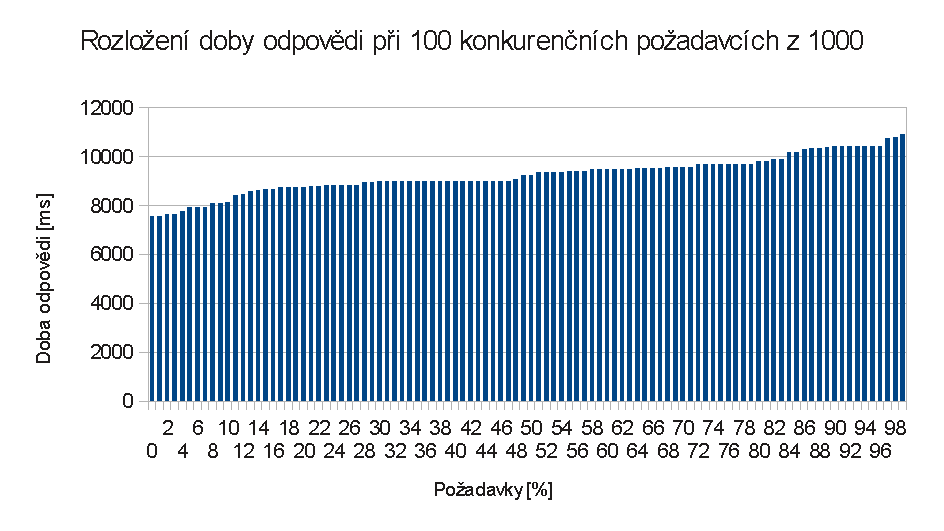
\includegraphics[width=12cm]{./figures/100-1000.pdf}
 % 100-1000.pdf: 453x255 pixel, 72dpi, 15.98x9.00 cm, bb=0 0 453 255
 \caption{Graf rozložení doby odpovědi}
 \label{fig:vykonnostniTesty}
\end{figure}

V průběhu testu nebyl pozorován znatelný nárůst spotřeby operační paměti, na druhou stranu systém vytížil přidělený procesor na maximum.

\subsubsection{Shrnutí testu}
Bylo ověřeno, že je možné provozovat systém bez jakýchkoliv obav, bude dostačovat pro předpokládaný provoz. Bohužel se mi nepodařilo zjistit, kolik souběžných požadavků by muselo být na server odesláno, aby vznikly vážné komplikace, z naměřených výsledků je ale patrné, že k tomu, mimo případy útoků, nikdy za stávajícího stavu nedojde.

V případě desíti požadavků za vteřinu, tedy s odezvou pod jednu vteřinu, uživatelé stále nepocítí žádné výkonnostní problémy, v případě sta požadavků za vteřinu, s odezvou pod deset vteřin, by dle \cite{PagesizeUseit} stále měli být schopní se soustředit na řešenou úlohu. Velmi pozitivní je nulová chybovost požadavků i~při vysoké zátěži.

Pokud by za nějakých nepředpokládaných okolností nastala situace vyžadující navýšení výkonu, lze postupovat jednou z následujících cest:
\begin{itemize}
 \item Přesunout systém z virtuálního stroje do plnohodnotného prostředí.
 \item Začít \textit{cachovat} odpovědi (téměř každá může být uložena a, při shodném dotazu v krátkém časovém horizontu, navrácena).
 \item Vhodněji indexovat databázi.
 \item Optimalizovat \glsname{SPARQL} endpoint.
 \item Distribuovat zátěž.
\end{itemize}
Předchozí cesty lze samozřejmě kombinovat a jejich výčet rozhodně není kompletní.


\subsection{Testování použitelnosti}
Na použitelnost (\textit{usability}) byl kladen důraz hlavně v případě mobilní aplikace, u serverové jsem se naopak použitelností příliš nezabýval -- nemá obsluhu, případně zaškoleného správce. Testování použitelnosti (\textit{usability testing}) bylo prováděno po celou dobu vývoje, formalizovaně ale až těsně před jeho dokončením, aby byla finální aplikace k uživatelům co nejpřívětivější.

\subsubsection{Charakteristika testu}
Testování probíhalo na čtyřech osobách podle následujícího scénáře: Účastníkovi byla předložena mobilní aplikace a byl mu ponechán čas na zběžné seznámení. V případě, že měl účastník vlastní vhodné zařízení, probíhalo testování na něm, jinak mu bylo poskytnuto jiné včetně pomoci s ovládáním, aby nebyly výsledky testu zbytečně zkreslovány. Poté byly účastníkovi zadány následující čtyři úkoly pokrývající předpokládané využití aplikace:
\begin{enumerate}
 \item[UT1] Vyhledejte pozici budovy T9. Úloha sleduje orientaci v základní struktuře aplikace.
 \item[UT2] Vyhledejte jídelníček menzy Masarykova kolej. Úloha sleduje schopnost využít průvodce.
 \item[UT3] Nacházíte se u vchodu to budovy T9, najděte nejbližší občerstvení. Úloha sleduje pokročilou obsluhu navigace.
 \item[UT4] Zjistěte si podrobnosti libovolného problému prostřednictvím \glsname{SPARQL} dotazu. Úloha sleduje schopnost využití \glsname{SPARQL} konzole.
\end{enumerate}
Po celou dobu byla osoba pozorována a po dokončení úkolů s ní byla provedena evaluace. Testování přineslo velký počet podnětů, které byly následně realizovány.

\subsubsection{Charakteristika účastníků}
Testování použitelnosti bylo provedeno na čtyřech účastnících charakterizovaných v tabulce \ref{tab:charakteristikaUcastniku}. % role účastníků
\begin{table}
\begin{center}
\begin{threeparttable}
\begin{tabular}{|c|c|c|c|c|}
\hline
\textbf{Osoba} & \textbf{Věk} & \textbf{Pohlaví} & \textbf{Povolání} & \parbox{2.2in}{\smallskip\textbf{Zkušenosti s počítačem, s~mobilním zařízením}\smallskip} \\
\hline
\textbf{P01} & 25 & žena & výzkum & \parbox{2.2in}{\smallskip pokročilá uživatelka, mírně pokročilá\smallskip} \\
\textbf{P02} & 23 & žena & studentka & \parbox{2.2in}{\smallskip pokročilá uživatelka, bez zkušeností\smallskip} \\
\textbf{P03} & 21 & muž & student & \parbox{2.2in}{\smallskip mírně pokročilý uživatel, bez zkušeností\smallskip} \\
\textbf{P04} & 21 & žena & studentka & \parbox{2.2in}{\smallskip občasná uživatelka, pokročilá\smallskip} \\
\hline
\end{tabular}
\caption{Charakteristika účastníků testování použitelnosti}
\label{tab:charakteristikaUcastniku}
\end{threeparttable}
\end{center}
\end{table}

\subsubsection{Průběh testu}
Osoby v tabulce \ref{tab:charakteristikaUcastniku} charakterizující účastníky testování jsou seřazeny chronologicky. Mezi jednotlivými testy byly ponechány krátké rozestupy, ve kterých jsem analyzoval jejich průběh a snažil se odstranit alespoň některé nalezené problémy -- jednotlivé průběhy tedy mezi sebou nelze příliš porovnávat.
\subsubsection*{P01}
\paragraph*{UT1}
Nejprve se snaží nalézt cestu k budově v sekci \textit{Průvodce}, po projití si ale uvědomuje, že by měla hledat v sekci \textit{Navigace} -- zpočátku ji považovala za mapu stránek. Poté hledaný objekt vyhledává posunem mapy.
\paragraph*{UT2}
Nalézá bez sebemenších problémů.
\paragraph*{UT3}
Snaží se nalézt občerstvení na mapě, nenalézá, přechází do sekce \textit{Průvodce}, opět nenalézá vrací se do \textit{Navigace}, ve vyhledávání zadává slovo \textit{bufet} a nalézá, pouze chvíli nevidí na mapě -- velmi malé a nevycentrované.
\paragraph*{UT4}
Nezná syntaxi dotazovacího jazyka \glsname{SPARQL}, prohlíží si ukázkový dotaz a vykonává ho.
\paragraph*{Poznámky}
Při pohybu na rozsáhlé úvodní stránce (nechala zobrazit příliš mnoho informací) se ztrácí v obsahu, nedaří se jí se jednoduše dostat nahoru k ovládání. Nečte nápovědu. Nevyužívá zpočátku vyhledávání u mapy.

\subsubsection*{P02}
\paragraph*{UT1}
Zpočátku ji nenapadá hledat v sekci \textit{Navigace}, vzápětí se tam ale přesouvá a budovu pohybem po mapě nalézá.
\paragraph*{UT2}
Nalézá bez sebemenších problémů.
\paragraph*{UT3}
Přechází do navigace, prochází mapou, občerstvení nenachází, zkouší ho proto vyhledat a nyní ho už nachází.
\paragraph*{UT4}
Nalézá záložku \glsname{SPARQL} a vykonává ukázkový dotaz, více se o \glsname{SPARQL} nezajímá.
\paragraph*{Poznámky}
Nečte nápovědu. Nevyužívá vyhledávání u mapy.

\subsubsection*{P03}
\paragraph*{UT1}
Ihned vstupuje do sekce \textit{Navigace}, mapou ale prochází manuálně, tlačítky -- ovládání gesty nezaregistruje. Nalézá.
\paragraph*{UT2}
Nalézá bez sebemenších problémů.
\paragraph*{UT3}
Přechází mezi sekcemi \textit{Navigace} a \textit{Průvodce}, nakonec používá vyhledávání, ve kterém nejprve zadává slovo \textit{vobčerstvení}, nakonec ale uznává, že použití slova \textit{občerstvení} bude mít větší šanci na úspěch a nalézá.
\paragraph*{UT4}
Vykonává předpřipravený dotaz a dále se o \glsname{SPARQL} nezajímá.

\subsubsection*{P04}
\paragraph*{UT1}
Sekci \textit{Navigace} nalézá okamžitě, budovu vyhledává, není si ale hned jistá, co je výsledkem -- v mapě se nezobrazilo překrytí okolí vyhledaného místa. 
\paragraph*{UT2}
Nalézá bez sebemenších problémů.
\paragraph*{UT3}
Občerstvení nalézá ihned, dále zkouší vyhledat slova \textit{bufet} a \textit{jídlo} a na obě také nalézá výsledky.
\paragraph*{UT4}
Vykonává předpřipravený dotaz a dále se o \glsname{SPARQL} nezajímá.

\subsubsection{Shrnutí testu}
Testování použitelnosti přineslo mnoho konstruktivních podnětů k vylepšení aplikace, naprostá většina se jich týkala navigace. Patří mezi ně především:
\subsubsection*{Motivovat k přečtení nápovědy}
Je vhodné motivovat uživatele k přečtení krátké nápovědy vysvětlující základní principy práce s aplikací. Všem účastníkům testování by to velmi prospělo. Může tak být učiněno například na webové stránce nabízející aplikaci ke stažení.
\subsubsection*{Našeptávání}
V průběhu testů použitelnosti byl na základě zpětné vazby od uživatelů realizován podstatně lepší vyhledávací algoritmus s našeptáváním.
\subsubsection*{Zvětšení vstupního pole navigace}
Vstupní pole vyhledávacího pole navigace bylo zvětšeno na základě dvou postřehů vyvstalých při testování použitelnosti: Pole bylo málo výrazné, takže uživatelé vyhledávání přehlíželi, a bylo poměrně malé, takže se do něj na dotykových zařízeních špatně trefovalo prstem.
\subsubsection*{Odřezání bílých znaků z okolí dotazu}
V průběhu testování byl několikrát nevědomky zadán k vyhledání výraz, který předcházel nebo následoval bílý znak, tudíž neodpovídal tomu v databázi, takže nebylo nic nalezeno. Problém jsem se rozhodl řešit odstraněním takových znaků.
\subsubsection*{Přesun na nalezené objekty}
Zpočátku uživatelé nezaregistrovávali nalezení hledaného objektu -- pouhé zobrazení šipky někde na mapě nebylo dostatečné. Implementoval jsem proto algoritmus pro přesun na vyhledávané místo a následné přeškálování mapy tak, aby byl zobrazen hledaný objekt i jeho okolí.
\subsubsection*{Odebrání tlačítka Centrovat}
Tlačítko pro vycentrování mapy se po přidání předchozí funkce ukázalo jako zbytečné -- uživatelé se už nemuseli při neúspěšném hledání nalezeného objektu vracet na původní místo, aby to zkusili od začátku, ale vyhledávaný objekt jim byl automaticky zobrazen.
\subsubsection*{Nápověda k regulárním výrazům}
Původně v nápovědě nebyla žádná zmínka o regulárních výrazech a jejich užití, ukázalo se to jako potřebné, proto byla přidána.
\subsubsection*{SPARQL konzole}
Potvrdilo se očekávání, že \glsname{SPARQL} konzole nebude patřit mezi nejoblíbenější funkce aplikace. Kdyby nebylo její užití testem přímo vyžadováno, nepoužil by ji nikdo. Z pohledu uživatelské přívětivosti by ji tedy bylo vhodné odstranit, neučinil jsem tak ale -- jedním z cílů práce je popularizovat nové důležité technologie mezi studenty a toto je vhodnou příležitostí k realizaci takového záměru.
% \subsubsection*{Fixní zobrazení menu}
% \subsubsection*{Legenda}

\pagebreak
\subsection{Srovnávací testování}
Srovnávací testování (\textit{comparative testing}) proběhlo pouze velmi zběžně -- neexistuje pravděpodobně totiž žádný jiný systém mající podobně specifické cíle. Pro potřeby testování jsem proto systém rozdělil na jednotlivé části tak, jak byly vyvíjeny -- serverovou a mobilní aplikaci. V případě serverové aplikace se mi nepodařilo objevit žádný konkurenční systém, na poli mobilních aplikací jich několik doménou obdobných již je, přesto je každá zaměřena na něco jiného.

Porovnávány byly aplikace Průvodce ČVUT FEL (\url{http://lr.czechian.net/j2me/}) a Studentův průvodce po fakultě (\url{http://webdev.felk.cvut.cz/~molnaja2/}). Je vhodné podotknout, že data první ze jmenovaných aplikací dávno pozbyla na platnosti a pro druhou aplikaci podklady pokrývající celou doménu ani nebyly vytvořeny. Za porovnání by určitě stály i vznikající aplikace z projektu ČVUT navigátor (\url{http://navigator.fit.cvut.cz/}), ty ale stále nejsou zveřejněny.

Vzhledem k výše uvedeným důvodům nebyla pro srovnání stanovena řádná metrika, ale je ponecháno na interpretovi, aby si z nalezených rozdílů vyvodil pro své potřeby patřičné závěry. Výsledky srovnání se nacházejí v tabulce \ref{tab:srovnaniReseni}.

\begin{table}
\begin{center}
\begin{threeparttable}
\begin{tabular}{|l|c|c|c|}
\hline
\tdh{Charak\-te\-ristika} & \tdh{Průvodce ČVUT FEL} & \tdh{Studentův průvodce po fakultě} & \tdh{Průvodce FIT ČVUT} \\
\hline
\tdh{Technologie} & \td{J2ME} & \td{XHTML, ECMAScript\dots} & HTML5 \\
\tdh{Platformy} & \td{Všechny s~Java~ME} & \td{Všechny s~webovým prohlížečem} & \td{Všechny s~lepším webovým prohlížečem} \\
\tdh{Stav vývoje} & \td{Předčasně ukončený 2006} & \td{Ukončený 2010} & \td{Ukončený 2010} \\
\tdh{Podklady} & \td{Jiné\tnote{a}} & \td{Jiné, malé\tnote{b}} & \td{Dostatečné\tnote{c}} \\
\tdh{Velikost (KB)} & \td{30} & \td{1900\tnote{d}} & \td{340\tnote{d}} \\
\tdh{Licence} & \td{Freeware} & \td{\glsname{GNU}/\glsname{GPL}v3} & \td{\glsname{GNU}/\glsname{GPL}v3} \\
\tdh{Průvodce} & \td{Navigace, dopravní spojení} & \td{Navigace} & \td{Navigace, studium, menzy, kontakty\dots} \\
\tdh{\color{dark}Objekty\linebreak navigace} & \td{Budovy, místnosti} & \td{Místnosti, body zájmu\tnote{e}} & \td{Budovy, místnosti, body zájmu\tnote{e}} \\
\tdh{\color{dark}Vyhledávání objektů} & \td{Označení místnosti} & \td{Označení místnosti, staré označení, zažitý název, jméno vyučujícího} & \td{Označení místnosti/budovy, neoficiální označení, body zájmu} \\
\tdh{\color{dark}Možnosti navigace} & \td{Popis, obrys budovy} & \td{Plán podlaží, \glsname{PCRE}} & \td{Plán kampusu/podlaží, aktuální pozice, \glsname{PCRE}} \\
\tdh{Další\linebreak vlastnosti} &  & Nápověda & \td{Nápověda, \glsname{SPARQL} konzole} \\
\hline
\end{tabular}
\begin{tablenotes}
 \item[a] Neaktuální. Budovy \glsname{FEL} \glsname{CVUT} -- T2, Z2, Z4, KN:E\dots
 \item[b] Pouze vzorek -- první a druhé podlaží na Karlově náměstí.
 \item[c] Rozsáhlý vzorek -- dejvický kampus nahrubo a první a třetí podlaží budovy T9 dopodrobna.
 \item[d] Velikost je brána z aktuálního stavu, s kompletními podklady naroste.
 \item[e] Občerstvení, toalety, výtahy\dots
\end{tablenotes}
\caption{Srovnání s ostatními mobilními aplikacemi}
\label{tab:srovnaniReseni}
\end{threeparttable}
\end{center}
\end{table}
